\documentclass[a4paper, 12pt]{article}
\usepackage[english]{babel}
\usepackage[utf8]{inputenc}
\usepackage[T1]{fontenc}
\usepackage{lmodern}
\usepackage{hyperref}
\usepackage[numbers, sort&compress]{natbib}
\usepackage{calc}
\usepackage{fancyhdr}
\usepackage{graphics}
\usepackage{nowidow}
\usepackage{color}
\usepackage{subcaption}
\usepackage{epsfig}
\usepackage{epstopdf}
\usepackage{verbatim}


\newlength{\eqMargin}
\newlength{\eqHorizMargin}
\newlength{\eqVertMargin}

\setlength{\eqMargin}{20mm}
\setlength{\eqHorizMargin}{\eqMargin}
\setlength{\eqVertMargin}{\eqMargin}

% Paper
\setlength{\paperwidth}{210mm}
\setlength{\paperheight}{297mm}

% Rid the extra space
\setlength{\hoffset}{-1in}
\setlength{\voffset}{-1in}
\addtolength{\hoffset}{\eqHorizMargin}
\addtolength{\voffset}{\eqVertMargin}

% Set margin from the page border (horizontal)
\setlength{\oddsidemargin}{0pt}
\setlength{\evensidemargin}{0pt}

% Header
\setlength{\topmargin}{0pt}
\setlength{\headheight}{42pt}
\setlength{\headsep}{18pt}
\renewcommand{\headrulewidth}{0pt}

% Footer
\addtolength{\footskip}{18pt}
\renewcommand{\footrulewidth}{0pt}

% Margin notes
\setlength{\marginparsep}{0pt}
\setlength{\marginparwidth}{0pt}

% Text
\setlength{\textwidth}{\paperwidth - \hoffset - \hoffset - 25.4mm - 25.4mm}
\setlength{\textheight}{\paperheight - \voffset - \topmargin - \headheight - \headsep - \footskip - \voffset - 25.4mm - 25.4mm}

%\setlength{\labelwidth}{20mm}

% Hyperref settings
\hypersetup{
    unicode=true,					% non-Latin characters in Acrobat's bookmarks
    pdftoolbar=true,				% show Acrobat's toolbar?
    pdfmenubar=true,				% show Acrobat's menu?
    pdffitwindow=false,				% window fit to page when opened
    pdfstartview={FitH},			% fits the width of the page to the window
    pdftitle={S-26.3120 Radio Engineering, laboratory course},	% title
    pdfauthor={Tuomas Leinonen} {Sampo Salo} {Huy Nguyen},	% author
    pdfsubject={Radio Engineering},	% subject of the document
    pdfcreator={LaTeX},				% creator of the document
    pdfproducer={Aalto},			% producer of the document
    pdfkeywords={radio} {gsm} {bs} {tx},	% list of keywords
    pdfnewwindow=true,				% links in new window
    colorlinks=true,				% false: boxed links; true: colored links
    linkcolor=black,				% color of internal links
    citecolor=black,				% color of links to bibliography
    filecolor=black,				% color of file links
    urlcolor=black					% color of external links
}

% Bad hyphenation
%\hyphenation{}

\definecolor{dkred}{rgb}{0.6, 0, 0}
\definecolor{dkgrn}{rgb}{0, 0.6, 0}
\definecolor{dkblue}{rgb}{0, 0, 0.6}

\pagestyle{fancy}
\lhead{S-26.3120 Radio Engineering, laboratory course\\Lab 2: GSM Base Station Receiver -- Final report\\}
\rhead{Sampo Salo, 79543L\\Tuomas Leinonen, 84695P\\Huy Nguyen, 411330}
\cfoot{\thepage}


\begin{document}

\begin{titlepage}
\pagestyle{empty}
\begin{center}

\vspace*{3cm}
\noindent\LARGE{\textbf{S-26.3120 Radio Engineering, laboratory course}}

\vspace*{2cm}

\Large{\textbf{Lab 2: GSM Base Station Receiver}}\\

\vspace*{1.5cm}

\large{\textbf{Final report}}\\
\vspace{1.5cm}
\large{\today}
	
\vspace*{3cm}
\large{
	\begin{tabular}{l l}
		\textbf{Group 3:} 	& \\
		Sampo Salo			& 79543L	\\
		Tuomas Leinonen 	& 84695P	\\
		Huy Nguyen			& 411330		
	\end{tabular}
}

\end{center}

\end{titlepage}


\section{Introduction}

TODO: Huy and Sampo (1st paragraph: general intro, 2nd: the measuremets, 3rd: structure of this report)

% ref:  (see Fig. \ref{fig:bs})

\begin{figure}[h!]
	\begin{center}
	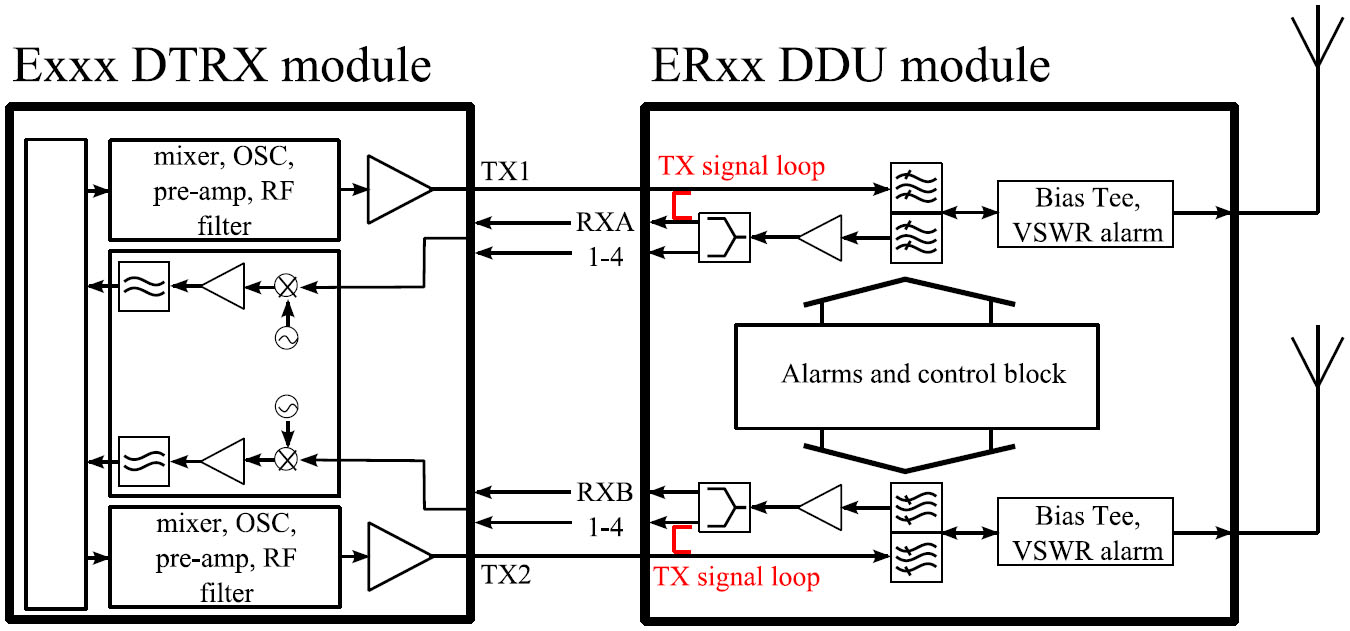
\epsfig{file=img/bs.jpg, width=\textwidth}
	\caption{Receiver under study.}
	\label{fig:bs}
	\end{center}
	\vspace*{-12pt}
\end{figure}


\newpage
\section{Measurement steps}

TODO: Tuomas

\begin{comment} % As an example
There were two types of measurements; power measurements with a spectrum analyzer 
(SA) and two-port measurements with a vector network analyzer (VNA). While the 
first three measurement tasks (i.e., $3.1 - 3.3$) were of the first kind, the 
last measurement (i.e., 3.4) was carried out using a VNA. The aforementioned 
measurement setups are described in detail in the following subsections, respectively. 
The setups correspond very closely to those presented in the pre-study.
\end{comment}


\subsection{1~dB compression point}

TODO: Tuomas


\subsection{Frequency response}

TODO: Tuomas

\begin{comment} % As an example
\begin{table}[!h]
	\begin{center}
	\caption{Two-ports measured with the VNA.}
	\label{tbl:2p}
	\renewcommand*{\arraystretch}{1.2}
	\begin{tabular}{ll}
	\textbf{Measurement} & \textbf{Two-port} \\
	\hline
	3.1 $-$ 3.3		& SMA-cable $+$ attenuator chain $+$ N-cable $+$ required adapters \\
	3.4 (a)			& $\mathrm{TX_B \rightarrow ANT_B}$ 	\\
	3.4 (b)			& $\mathrm{TX_B \rightarrow RX_{B1}}$ 	\\
	3.4 (c)			& $\mathrm{ANT_B \rightarrow RX_{B1}}$
	\end{tabular}
	\end{center}
	\vspace*{-12pt}
\end{table}
\end{comment}


\subsection{Noise temperature}

TODO: Tuomas

\subsection{Sensitivity}

TODO: Tuomas


\newpage
\section{Results}

TODO: Huy and Sampo (general results and intro to more specific results)


\subsection{1~dB compression point}

TODO: Huy and Sampo


\subsection{Frequency response}

TODO: Tuomas


\subsection{Noise Temperature}

TODO: Huy and Sampo


\subsection{Sensitivity}

TODO: Huy and Sampo


\subsection{Dynamic range}

TODO: Huy and Sampo


\newpage
\section{Error estimates}

TODO: Huy and Sampo (make additions, corrections, change the style to avoid excess 
repetition etc.)

In this section, error estimates for the two types of measurements are presented.
The values presented here are only rough estimates based on literature (with more 
or less general cases) and their soundness in this case is somewhat questionable. 
In this section, we do not take human errors (see previous section) into account. 
It is just stated that systematic errors arising from the cables and connections 
are possible in measurement all measurements. Thus they are valid only for 
``correct'' measurements, and are more of the ``provided for completeness'' 
nature. Probabilities are not given due to the nature/basis of the estimation.


\subsection{Spectrum analyzer}

Each of the components inside the spectrum analyzer contributes to the total uncertainty, 
depending for example on the signal frequencies, amplitudes, and measurement settings. 
The Agilent (former HP, manufacturer of the used SA) has made available a document that 
specifies the different error sources, giving also rough estimates for some spectrum 
analyzers. According to the document \cite{sa}, the error estimates vary broadly among 
different analyzer models, giving worst case uncertainties exceeding $\pm 6$ dB. On the 
other hand, the document gives also representative values of amplitude uncertainties, 
which in our case yields about $\pm 1$ dB.

The second error source for the spectrum analyzer is the power marker reading. In 
each of the tasks, the spectrum analyzer was set to average 500 measurement points, 
which should average out most of the random errors. However, reading the power marker 
in the screen, there was a noticeable fluctuation in the shown power value. Based on the 
experience obtained during the measurements, the power marker error is estimated to be 
approximately $\pm 0.5$ dB.

In conclusion, the error estimates that can be taken into account numerically are 
the manufacturers representative value of approx. $\pm 1$ dB, and the power marker 
fluctuation of roughly $\pm 0.5$ dB. These uncorrelated errors may be summed to 
achieve the total uncertainty of the SA measurements of approx. $\pm 1.5$ dB. 

There is also the question of calibrating the spectrum analyzer properly with 
the time interval defined by the manufacturer. Agilent suggests to have the spectrum 
analyzer calibrated thoroughly once in a year, and quick-calibrated if there are 
changes operating environment \cite{sa2}. If the spectrum analyzer used in the 
measurements is not calibrated correctly, it is possible that the measurements are 
not reliable. In this case, the calibration is the most important error source, and 
the device should be calibrated correctly before estimating any other errors.


\subsection{Vector network analyzer}

For the VNA, different error sources and ways to cope with them are listed in the 
lecture slides discussing VNA measurements. The different sources are noise, 
cabling/connector repeatability, directivity, isolation, mismatch and environment 
induced drift. 

Noise and cabling/connector repeatability are random errors, which can be averaged 
out. In our case, only the noise was averaged, since we did not touch the cabling. 
Systematic errors arising directivity, isolation, and mismatch in this task were
for the most part neglected with a calibration. Before conducting measurements, 
the VNA is always calibrated using a standard calibration module. The calibration 
moves the reference planes to the connectors of the test cables, and somewhat 
cancels the systematic errors from the connectors and cables used in a specific 
measurement. Finally, the environment induced drift is not relevant, since the 
measurement was done inside a short time interval.

Rohde \& Schwarz provides specifications that describe the measurement uncertainty 
of the VNA in question in different frequency bands. For transmission measurements 
in the frequency range of 50 MHz to 3 GHz, accuracy for signal powers of $-50 \ldots 0$ 
dB is better than $0.2$ dB ($0.3$ dB for powers of $-50 \ldots {-70}$ dB) with 0 dBm 
transmit power. \cite{vna} The reader should note that these ranges was exceeded 
from both ends during the measurements (the measurement power range was roughly 
$-100 \ldots {+4}$ dBm). 

In conclusion, two things are assumed. First, calibration is assumed to cancel the 
systematic errors arising from cables and connectors. Second, random errors are 
cancelled with averaging. The manufacturer provides error estimates for the device 
itself, giving an error estimate of under $0.3$ dB that is mostly applicable in 
our case. The topics discussed in the last paragraph of the last subsection apply 
here to some extent to here as well.


\newpage
\section{Conclusions}

TODO: Huy and Sampo


\newpage
\section{Feedback}

TODO: Huy and Sampo


\newpage
\begin{thebibliography}{9}%\itemsep 7pt\parskip -5pt 

\bibitem{lab2} C.\ Icheln, S.\ Khanal, 
	\textit{GSM Receiver laboratory assignment instructions},
	S-26.3120 Laboratory course in Radio Engineering course material.
	
\bibitem{} C.\ Icheln (edited), 
	\textit{Lecture supplement handout},
	S-26.3120 Laboratory course in Radio Engineering course material.

\bibitem{sa} Agilent, Spectrum Analysis Basics, Application Note 150. 
	Available online at \url{http://cp.literature.agilent.com/litweb/pdf/5952-0292.pdf} 
	[Retrieved: Jan 2nd, 2014].
	
\bibitem{sa2} Agilent, 8590 Series Analyzers Calibration Guide.
	Available online at \url{http://cp.literature.agilent.com/litweb/pdf/08594-90106.pdf}
	[Retrieved: Jan 2nd, 2014].
	
\bibitem{vna} R\&S ZVL Vector Network Analyzer Specifications, 
	Version 06.00, Dec 2008. 
	Available online at \url{http://www.upc.edu/pct/documents_equipament/d_160_id-655-2.pdf} 
	[Retrieved: Jan 2nd, 2014].


%\bibitem{pozar} D.\ M.\ Pozar, 
%	\textit{Microwave Engineering}, 
%	J.\ Wiley \& Sons, 4th Edition, 2012. 
%	ISBN: 978-0-470-63155-3.
	
%\bibitem{gains} J.\ C.\ Logan, J.\ W.\ Rockway, 
%	``Dipole and Monopole Antenna Gain and Effective Area for Communication Formulas.''
%	Available online at \url{www.dtic.mil/cgi-bin/GetTRDoc?AD=ADA332891}
%	[Retrieved: November 25, 2013].

%\bibitem{parts} M.\ Steer, 
%	\textit{Microwave and RF Design -- A Systems Approach}, 
%	SciTech Publishing, 2010. 
%	ISBN: 978-1-891-12188-3.
	
%\bibitem{iet} R.\ J.\ Collier, A.\ D.\ Skinner (editors), 
%	\textit{Microwave Measurements}, 
%	The Institution of Engineering and Technology, 3rd Edition, 2007. 
%	ISBN: 978-0-86341-735-1.

\end{thebibliography}

\end{document}
